L'electrònica s'encarrega de rebre i processar el senyal elèctric emès pel fotosensor i d'emmagatzemar la informació pertinent. Les diferents tasques realitzades per l'electrónica són aplicar llindars energétics sobre el senyal (utilitzats per descartar senyals no perteneixents a esdeveniments de triti), amplificar el senyal (per tindre millor precisió en les operacions realitzades sobre aquest) i aplicar coincidencies (per reduir la quantitat d'esdeveniments no perteneixents al triti). Finalment es realitza un histograma dels senyals que han superat totes les etapes anteriors, obtenint un espectre amb l'informació d'interés (l'energía dels esdeveniments). 

L'electrónica depén del tipus de senyal que reb i, per tant, del tipus de fotosensor utilitzat. A causa d'això, en la col·laboració TRITIUM s'utilitzen electróniques diferents, una per a les matrius de SiPMs i altra per a els PMTs:

\begin{enumerate}

\item{} L'electrónica emprada per a quan s'utilitzen matrius de SiPMs s'anomena PETsys \cite{PETSYS}, mostrada a la Figura \ref{fig:PETSYSs}, un sistema comercial desenvolupat específicament per a treballar amb matrius de SiPMs. 

\begin{figure}[h]
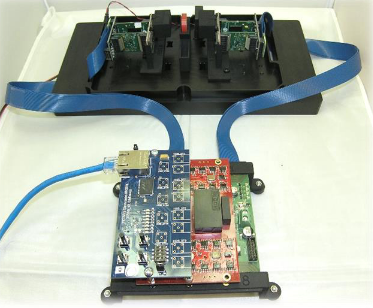
\includegraphics[scale=0.5]{12Summary/3DesignPrinciples/32Tritium_detector/PETSYS_System.png}
\centering
\caption{Sistema comercial PETsys\label{fig:PETSYSs}.}
\end{figure}

\item{} L'electrónica emprada quan s'utilitzen PMTs és diferent depenent de si aquests van a ser utilitzats en el laboratori o en Arrocampo, l'emplazament final del detector. Per als experiments de laboratori es fa servir la tecnología NIM, la qual és un tipus de tecnología modular i interconectada. Per als experiments en Arrocampo, l'equip portugues de la col·laboració TRITIUM va disenyar i construir una electrònica específica que està basada en diverses tarjetes de circuit imprés (PCB per les sigles en anglés).

\end{enumerate}